In this Chapter we introduce the models and assumptions this work is based on.
% we  introduce  some  of  the  notation  that  wewill  use  throughout  the  paper
We define the system and data model that we consider in this work (Section~\ref{sec:models}),
and discuss the requirements guiding the design of query processing systems (Section~\ref{sec:requirements}).

\section{Models}
\label{sec:models}
We consider a data serving system with a two-tiered architecture: a data storage tier and a query processing tier.

\begin{itemize}
  \item The data storage tier is responsible for storing and providing access to data.
  We use the terms \textit{storage system} or \textit{data store} to refer to the system that implements this tier.

  \item The query processing tier is responsible for providing the functionality to identify and retrieve data using
  queries on secondary attributes (Section~\ref{subsec:query_prcessing_tier}).
  We refer to the system that implements this tier using the terms \textit{query engine} or \textit{query (processing) system}.
\end{itemize}

\begin{figure}
  \centering
    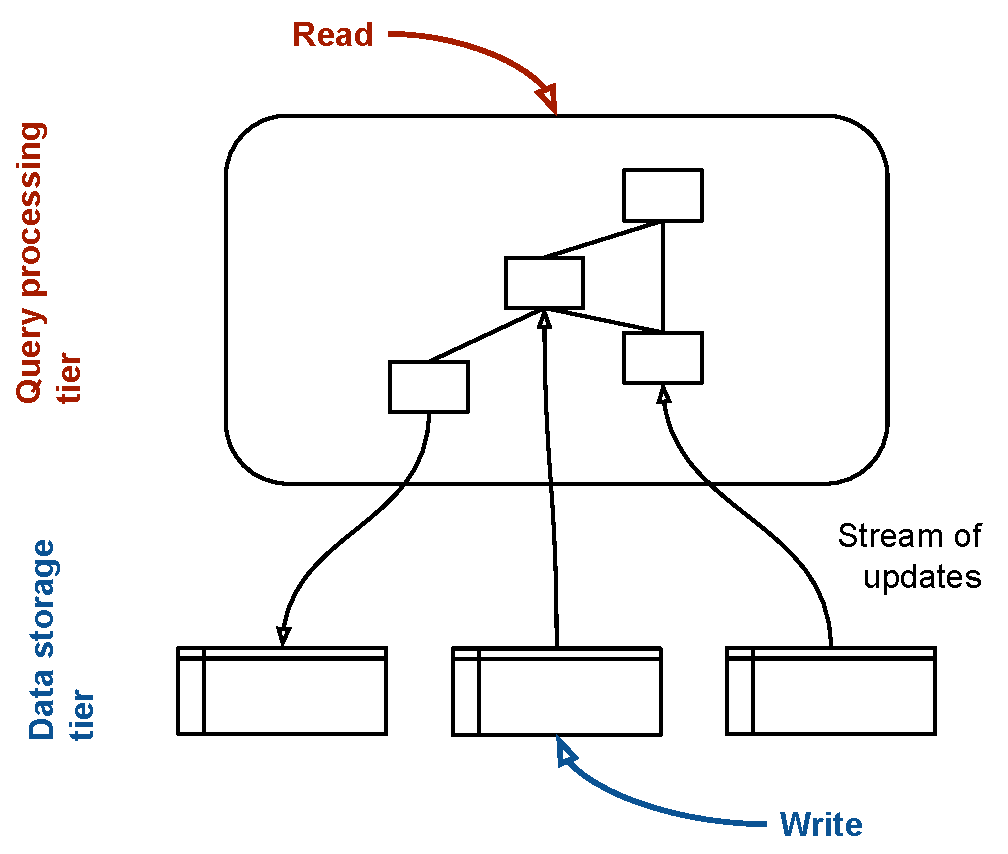
\includegraphics[width=0.5\textwidth]{./figures/models/data_flow.pdf}
  \caption{An overview of the system model.}
  \label{fig:high_level_dataflow}
\end{figure}

\noindent
Figure~\ref{fig:high_level_dataflow} shows a high level overview of the system model

\begin{itemize}
  \item A user submits an \textit{update operation} to the data storage tier.
  As a result, data flows from the user to the data storage tier, and then optionally to query processing tier.
  The query processing tier may use this data to update data structures such as secondary indexes and materialized views.

  \item A user submits a query to the query processing tier.
  As a result, control messages linked to the query execution flow through the query processing tier, and potentially
  for the query processing to the data storage tier (a query processed using cached data does not require control flow
  between tiers, while a query that requires reading from base tables does).
  Data --- in the form of intermediate or final query results flow from the storage tier to the query processing tier to
  the user.
\end{itemize}

\medskip
\noindent
Disaggregating query processing from the storage engine is an approach used by various systems and cloud
services such as Amazon Athena \cite{aws:athena}, Aurora \cite{aws:aurora}, and Google BigQuery
\cite{google:bigquery}.
In these systems, query processing is performed by a query engine independent from the storage system.

This model provides several benefits:
\begin{itemize}
  \item It enables application infrastructures to run a mix of different query workloads on the same data,
  without the need to move data to different systems in order to take advantage of their query processing capabilities.

  \item Storage and query processing resources can scale independently.
  The query engine can elastically adapt to match the query processing requirements of time-varying workloads,
  without over provisioning resources \cite{vuppalapati:elasticqueryengine}.

  \item It enables ad-hoc, one-time queries on already existing data without the need to migrate data.
  For example, performing log forensic queries for incident investigation.

  \item It enables cloud providers to implement fine-grained pricing for querying services.
\end{itemize}

\medskip
\noindent
In this work, we focus on the design of the query processing tier and consider the data storage tier as ``imposed'';
We consider the data storage tier's functionalities, guarantees, and data distribution schemes as input parameters in
our design.

% The bidirectional flow of data and control messages the fundamental property of the presented system model, and guides our query processing tier design, as discussed in section \todo{}.

\subsection{Data storage tier}

The data storage tier is a broad abstraction which includes any system that can be used to store and retrieve data.
This can include databases, file systems, cloud object storage systems.

As described above, in this work we view this tier as an external, underlying system that our design can build upon.
However, any efficient query processing tier design needs to take into account the properties and characteristics of the
data storage tier, most importantly its data distribution scheme.
To address this, we adopt a narrower data storage tier definition.
More specifically, we model a data storage tier as a federation of geo-replicated storage systems.
In the following section, we present our data storage tier model in detail.


\subsubsection{System model}
The data storage tier is implemented by a storage system (a database, file system or cloud storage system) or a
\textit{federation} of multiple, potentially heterogeneous storage systems.

Each system is responsible for storing a large dataset $D$, continuously updated by a stream of small changes.
We use the term \textit{corpus}  --- usually used in the information retrieval literature to refer to a collection of documents ---
to refer to the entire collection of data stored by the data storage tier.

We model the storage systems that can be used to implement the storage tier as distributed, replicated partitioned systems \cite{agrawal:taxonomy}.
% A Taxonomy of Partitioned Replicated Cloud-based Database Systems
In order to improve scalability, the dataset is divided into non-overlapping parts (usually call partitions or shards),
so that each partition can be managed by a separate system node.
Moreover, to improve availability, each partition is replicated.
We consider both full replication, in which each replica is a complete copy of the dataset,
and partial replication, in which a replica might be a copy of a subset of the dataset.

Finally, we consider federated systems that provide a unified namespace over multiple independent datasets stored in different storage systems.

\medskip
\noindent
We model the infrastructure on which the data storage tier runs as a collection of \textit{sites}.
A site is a group of nodes (servers, user devices) with the following characteristics:
\begin{itemize}
  \item Network communication latency between nodes in different sites is significantly higher (typically an order of
  magnitude higher) \cite{pbailis:hats} compared to communication latency within a site.
  \item Network bandwidth is high within a site and more limited and costly across sites.
  This is reflected in the pricing for cross-region data transfer in public cloud platforms.
  Using the AWS Pricing Calculator \cite{aws:costcalc} we see that data transfer to different AWS data centers
  (regions) costs double the price of intra-DC data transfer (0.02 and 0.01 USD per GB respectively).
\end{itemize}

A site can correspond to a data center, a group of servers serving as an edge Point of Presence \cite{google:infra}, or
a group of user devices in close proximity (in the same room or building).

\subsubsection{Data model}
We define the corpus as a collection of \textit{data items}, organized in \textit{tables}.
We use the term \textit{data item} to refer to the unit of stored data:
Depending on the semantics of the storage system that implements the data storage tier,
a data item may correspond to a file, an object, or a database record.
Tables may be organized in a hierarchical structure (file system directories), a flat namespace (object store buckets),
or in a relational schema.

A data item is composed of a primary key, a set of attributes, and a value (or content).
The primary key can be used to \textit{efficiently} identify and retrieve data items, without requiring a scan.
Attributes are key-value pairs.
We do not assume a strict schema for attributes: the attributes of each data item are independent of the attributes of
others.
Finally, a data item's value can be any sequence of bytes, such as an image, video, or PDF file.

Our main focus is on data item attributes.
We consider data item attributes to be mutable.
The data storage tier provides clients with operations for inserting and removing data items,
modifying the attributes of a specified data item, and retrieving the attributes of a given data item.

% should we differentiate the value? having the content as a normal attribute creates the assumption that it can be part of query processing as any other attribute.
% We haven't considered in our design consideration of image / video / ... search
\medskip
\noindent
This data model can express the data models of multiple different types of storage systems:
\begin{itemize}
  \item Object stores, such as AWS S3: \\
  The data storage tier is implemented as an object store.
  In that case, a data item corresponds to an object and a tables to a bucket.
  The data item's value corresponds to the object's content,
  and attributes correspond to object tags \cite{awss3:tagging}.

  \item Wide-column stores, such as Amazon DynamoDB, Google's Bigtable or Apache Cassandra: \\
  In a data storage tier implemented by a wide-column store:
  \begin{itemize}
    \item Data is organized in tables.
    \item Data items correspond to table rows and attributes correspond to columns.
  \end{itemize}

  \item Relational databases: \\
  In a data storage tier implemented by a relational database each table record corresponds to a data item, and each
  table column corresponds to an attribute.
  The relational schema can be represented by enforcing a corresponding schema for the attributes of data items in each
  table.

  \item Document-oriented databases: \\
  Document-oriented databases (or document stores) structure information in the form of documents (semi-structured data).
  Documents encode data in some standard format such as XML, YAML, JSON or BSON.

  The described data model is partially compatible with the document store data model:
  tables correspond to document collections, and data items correspond to documents.
  A document's identifier can be represented as a data item's primary key, while document attributes can be represented
  as attributes.
  However, the data model presented in this section cannot express complex attribute types such as lists and maps,
  or nested attributes which are used in the formats used in document stores.

  \item File systems: \\
  In a data storage tier implemented by a file system, data items correspond to files and tables correspond to file
  system directories.
  A data item's primary key corresponds to the corresponding file's path, the value to the file's content,
  and attributes correspond to extended file attributes.
\end{itemize}

This general data model, which is able to express different existing data models, satisfies the design goal mentioned
above:
Allowing the query processing tier to be independent from the underlying data storage tier, and be compatible with
different storage tier implementations.

\medskip
\noindent
\textbf{Timestamps} \\
We assume multi-version storage.
Each data item is associated with a timestamp.
Modifying the value of a data item's attribute, creates a new version of the data item,
which is associated with the timestamp assigned to the operation that resulted to it.
Timestamps can be implemented using any data type that provides a partial or total order, such as Unix time or vector timestamps.

\medskip
\noindent
In summary, we model a table as a collection of tuples of the form:
\[
  (PrimaryKey,~[(AttributeName,~AttributeValue)],~Timestamp)
\]
\begin{sloppypar}
Each tuple represents a data item version.
$PrimaryKey$ is the data item's primary key, $[(AttributeName,~AttributeValue)]$ is an array of attribute names and values
representing the data item's attributes, and $Timestamp$ is the timestamp associated with that version.
\end{sloppypar}

\subsubsection{Data storage tier API}
One of our design decisions (section~\ref{sec:design_rationale}) is to design the query processing tier as a middleware
system, decoupled from the data storage tier.
Moreover, we require the query processing tier to be able to interoperate with multiple different data storage tier implementations.

To achieve that, we model the interconnection between the data storage and query processing tier as a set of well-defined APIs.
This allows the query processing tier to be compatible with any data storage tier implementation that exposes these APIs.

% As an example, the query processing tier can work on top of a streaming system that does not persist data but exposes the $Subscribe$ API.

To be compatible with our design, a data storage tier needs to expose some the following APIs:
\begin{itemize}
  \item An API for iterating over the corpus data (List).
  This API enables the query processing tier to access corpus data.
  It can be used to implement query processing tasks such as iterating over a table's data items and filtering those that
  match a given predicate, or performing a join over two tables.

  \item An API for subscribing to notification for changes to the corpus data (Subscribe).
  This API enables the query processing tier to receive a constant stream of notifications for corpus data changes,
  which can be used to incrementally maintain data structures such as indexes and materialized views.
  % \item An API for querying the corpus data (Select).
  % This API allow the query processing tier to make use of the querying capabilities of the data storage tier.
\end{itemize}

% List and Subscribe are complementary, and are both needed for a fully featured query processing tier.
% Select is optional;
% It models querying capabilities provided by the data storage tier.
% , as it can be viewed as a generalization of List (a List is a Select without predicates)

% In short:
% \begin{itemize}
%   \item When only the List API is available, the query processing tier can perform any querying task, but the use of
%   derived data for optimizations is limited.
%   The query processing tier can build indexes and materialized views by scanning the corpus data, but updating those data
%   structures to reflect corpus data changes requires a full rebuild.

%   \item When only the List API is available, the query processing tier can perform query processing tasks only by
%   building a derived view of the corpus data (build materialized views).
%   Depending on the semantics of Subscribe, the query processing tier may only be able to receive information for corpus
%   updates with timestamps starting from the invocation of the Subscribe API, making the query processing tier not
%   possible to deploy over already existing data.
% \end{itemize}
For the rest of this document,
we make the assumption that the data storage tier provides the List and Subscribe APIs as describe below.
In section \todo{ref chapter 5}, we discuss the implications providing a subset of the APIs described in this section,
such as providing only List or Subscribe, or not exposing data object versions.
In section \ref{sec:implementation} we comment on the implementation the storage tier APIs using the functionalities of existing data storage systems.

\bigskip
\noindent
\textbf{API 1: List}

\noindent
The List API provides a mechanism for retrieving a set of versions of every object in a given table:

\[
  List(Table, [Timestamp_{low}, Timestamp_{high})) \rightarrow [ListResponse]
\]

\noindent
\begin{sloppypar}
Given a table name ($Table$) and a time internal, expressed as range of timestamps ($[Timestamp_{low}, Timestamp_{high})$),
$ListResponse$ contains all data item versions in $Table$ with $Timestamp_{low} \leq Timestamp < Timestamp_{high}$.
\end{sloppypar}

We do not assume specific semantics for $ListResponse$.
For example it may be implemented as a single response containing an array of response entries,
as a stream in which each entry is sent as a stream record,
or an iterator in which calling a $Next()$ method returns the following response entry.

Finally, we do not assume any ordering in $ListResponse$.

% The $List$ API may be provided as an explicit API method or enabled as a composition of other APIs, such as a combination of a \textit{list} and a \textit{read} (get) operation.

% Depending on its versioning mechanism, the storage system implementing the data storage tier may not support the
% listing API for any range of timestamps.
% For example, in a storage system that does not provide multi-versioned storage, $List$ will return the latest version of
% each data item.
% For simplicity, we assume the $List$ API as specified above.
% In Section \todo{}
% we describe how our design can use the $List$ API without support for Timestamp ranges.

\bigskip

\noindent
\textbf{API 2: Subscribe}

\noindent
The Subscribe API provides a mechanism for subscribing to notification for updates to data items in a given table:

\[
  Subscribe(Table, [Timestamp_{low}, Timestamp_{high})) \rightarrow [SubscribeResponse]
\]

\noindent
\begin{sloppypar}
Given a table name ($Table$) and a time internal,
$SubscribeResponse$ contains an entry corresponding to each update performed in a data item $d$ in $Table$, with
$Timestamp_{low} \leq Timestamp < Timestamp_{high}$.
$SubscribeResponse$ entries are of two types.
\textit{Creation} entries have the structure $(PrimaryKey,~[(AttributeName,~AttributeValue)],~Timestamp)$.
\textit{Deletion} entries have the structure $(PrimaryKey,~Timestamp)$.
A creation entry represents an inserts operation that creates new a data item,
while a deletion entry represents a delete operation.
An operation that modifies the value of a data item's attribute is represented by a creation entry followed by a deletion
entry.
\end{sloppypar}

$SubscribeResponse$ has streaming semantics:
An invocation of $Subscribe$ returns a stream handler;
The storage tier emits records at the stream corresponding updates performed to the corpus.

Various systems provide mechanisms that can be used to implement the $Subscribe$ API.
Examples include triggers in traditional database management systems \cite{mariadb:triggers}, and event notification
mechanisms in cloud storage services \cite{awss3:notifications}.

% \bigskip

% \noindent
% \textbf{API 3: Select}

% \noindent
% This API provides a mechanism for identifying data items based on their attributes:

% \begin{sloppypar}
% \[
%   Select(Table, Predicate, [Timestamp_{low}, Timestamp_{high})) \rightarrow [SelectResponse],
% \]
% where $Predicate$ is a map containing attribute keys and ranges:
% $\{AttrKey: [AttrVal_{low}, AttrVal_{high})\}$.
% \end{sloppypar}

% \begin{sloppypar}
% Given a table name ($Table$), a range of timestamps ($[Timestamp_{low}, Timestamp_{high})$), and
% a predicate consisting of attributes keys and ranges of values
% ($\{AttrKey: [AttrVal_{low}, AttrVal_{high})\}$), $Select$ returns $SelectResponse$.
% $SelectResponse$ contains all data items in $Table$ that have all attributes contained in $Predicate$ and
% their values are within the ranges specified in $Predicate$.
% \end{sloppypar}

% $Select$ can be expressed as an SQL query with the form: \\
% \noindent
% $SELECT$ $AttrKey_1$, $AttrKey_2$, ..., \\
% $FROM$ $Table$ \\
% $WHERE$ \\
% $AttrKey_1$ $IS$ $NOT$ $NULL$ $AND$ $AttrVal_{low}$ $\leq$ $AttrKey_1$ $<$ $AttrVal_{high}$
% $AND$ $AttrKey_2$ $IS$ $NOT$ $NULL$ $AND$ $AttrVal_{low}$ $\leq$ $AttrKey_2$ $<$ $AttrVal_{high}$
% $AND$ ... \\
% $AND$ $Timestamp_{low}$ $\leq$ $Timestamp$ $<$ $Timestamp_{high}$

% $Select$ may be provided as a subset of a more expressive query language, such as in relational database
% systems that support a full SQL query language. \\

\subsection{Query processing tier}
\label{subsec:query_prcessing_tier}
Τhe main focus of this work are the design decisions and trade-offs involved in the design of the query processing tier.
In this section we present an overview of the query processing tier's role and functionality.
In the following chapters we review the known approaches and techniques for building a query processing tier (Chapter~\ref{ch:background},
examine the design decisions and associated trade-offs involved in the design (Chapter~\ref{ch:design_space}),
and finally present our query processing tier design (Chapters~\ref{ch:design_pattern} and~\ref{ch:proteus}).

\medskip
\noindent
The query processing tier is responsible for providing attribute-based data retrieval.
It provides a $Query$ operations which client can user to retrieving data items using queries on their attributes.


\subsection{Query language}

We consider a query language that supports selection, projection, aggregation and join operators.
We consider supporting an extensive query language to be out of the scope of this work.
We argue that this query language is expressive enough to support a variety of applications,
and simple enough to allow this work to focus on the architecture design of the query processing tier.

\begin{itemize}
  \item The selection operator is defined as:
  \[
  Selection(Table,~AttributeName,~Operator,~Value)
  \]
  where Operator is a binary operator in the set $\{<,~\leq,~=,~\neq,~>,~\geq,~>\}$,
  and $Value$ is a constant specifying a value.
  $Selection$ denotes all data items in $Table$ which
  have an attribute $AttributeName$,
  and for which $Operator$ holds between the value of attribute $AttributeName$ and the constant $Value$.

  Moreover, queries can combine multiple $Selection$ operators with logical operators.
  For example, the query:

  \begin{lstlisting}
  SELECT order_id
  FROM Orders
  WHERE status != "shipped" AND order_date <= 10-10-2020
  \end{lstlisting}

  specifies an \textit{attribute predicate} using the conjunction of two $Selection$ operators.

  \item The projection operator is defined as :
  \[
  Projection(AttributeName_0,~AttributeName_1,~...)
  \]

  $Projection$ operates in the set of attributes associated with a data item.
  The result of a projection operation over a data item, is the data item with its attribute set restricted to the
  intersection between the attributes specified by the projection, and the attributes associated with the data item.

  \item An aggregation operator is defined as
  \[
  Aggregation(Table,~Function,~AggregationAttribute,~GroupingAttribute)
  \]
  where $Function$ is a function in the set $\{COUNT,~SUM,~AVERAGE,~MAX,~MIN\}$,
  and $OperandAttribute$ and $GroupingAttribute$ are attribute names.
  $Aggregation$ groups the data items in $Table$ in groupings based on their value of $GroupingAttribute$,
  and, for each group, applies $Function$ to the values of $AggregationAttribute$.
  The result of an aggregation function is a new table that contains a data item for each aggregation group.
  Each data item contains the result of the aggregation function as an attribute, and has the value of the grouping attribute as primary key.

  \begin{lstlisting}
  SELECT customer_id, SUM(amount)
  FROM Orders
  GROUP BY customer_id
  \end{lstlisting}

  groups the data items in Orders based on the value of the $customer\_id$ attribute,
  and applies the SUM function to the $amount$ attribute of every data item in each group.

  \item The join operator is defined as
  \[
  Join(BaseTable,~JoinTable,~JoinAttribute)
  \]
  where $BaseTable$ and $JoinTable$ are two corpus tables, and $JoinAttribute$ the attribute on which to perform the join.
  $Join$ performs a left outer join.
  The join results contains all data items in $BaseTable$.
  For each data item in $BaseTable$, the operation examines the $JoinTable$ for \textit{matching} data items.
  A matching data item is one that has the same value as the base data item for the $JoinAttribute$.
  If a matching data item existing for a base data item, then the join result for this data item contains the union of the attributes of the two.

  We consider this type of join operation in our query model because it has been shown to be useful to application that
  model their data using semi-structured data \cite{mongodb:joins}.
\end{itemize}


% The interface supports a query language with an SQL-like syntax.
% The query language supports point and range queries, logical operators, aggregation functions, and joins.
% We argue that these is no inherent limitation in the QPU model that prevents it from supporting a more complex query language (for example supporting nested queries).
% However, we consider additional functionalities to be out of the scope of this work.
% We believe this query language can effectively demonstrate that the QPU model can be used as building
% block for constructing fully-functional query processing systems.


% As the query language, we consider the subset of SQL that supports expressions of the form: \\

% \noindent
% $SELECT$ $projection$ $FROM$ $Table$ $WHERE$ $predicate$,

% \noindent
% where
% \begin{itemize}
%   \item $projection$ is a list of attributes, $AttrKey_1$, $AttrKey_2$, ..., $AttrKey_N$.
%   \item $predicate$: has the form: \\ $rangePredicate_1$ $AND$ $rangePredicate_2$ $AND$ ... $AND$ $rangePredicate_N$, \\
%   where $rangePredicate_i$ an expression of the form $AttrVal_{low}$ $\leq$ $AttrKey$ $<$ $AttrVal_{high}$.
% \end{itemize}

% \todo{this needs some work to define exactly what is and is not supported (we now support more than previous iterations, for example some simple joins)}

% Given a query $Q$ = ($projection$, $table$, $predicate$)
% and a data item $d$ = ($table$, $id$, $attributes$), $d$ satisfies $Q$ if:
% \begin{itemize}
%   \item $Q.table$ = $d.table$: the data item belongs in the table referred by the query, and
%   \item $\forall$ ($AttrVal_{low}$ $\leq$ $AttrKey$ $<$ $AttrVal_{high}$) $\in$ $Q.predicate$:
%   $attrKey$ $\in$ $d.attributes$ and $AttrVal_{low}$ $\leq$ $AttrVal$ $<$ $AttrVal_{high}$:
%   the data item contains all attributes included in the query's predicate, and their values are within the ranges
%   specified by the predicate.
% \end{itemize}

% $Predicate$ may contain expressions that refer to the $Timestamp$ predicate.
% In that case, a data item satisfies $Q$ if, in addition to the above conditions, its $Timestamp$ satisfies the
% $Timestamp$ -related expressions in $predicate$.
% If no $Timestamp$ -related predication is given, then only the latest version of each data item is considered for the
% query.

\noindent
We define the set of data items that satisfy a query $Q$ as $Q_r$.
In the ideal case, $Q$'s response is $Q_r$, however, as we explain in the following section a query response may
differ from $Q_r$.

\subsection{Derived data}
Query systems often maintain data such as indexes, materialized views, and caches.
We refer to this data as \textit{derived} data.
Derived data, in the general case, is obtained by performing a computation over the base data.
When base data changes, the query system need to update derived data to reflect theses changes.
After a base data updates, indexes and materialized views need to be update so that the reflect the new state of the corpus,
and obsolete cache entries need to be invalidated.
As we describe in the following section, inconsistencies between base and derived data may result to divergence between
query responses and $Q_r$, as $Q_r$ is defined using the most up-to-date state of the corpus at the time of a query, but
query processing may be based on an outdated view of the corpus data.

\section{Query processing system performance evaluation}
\label{sec:requirements}

% An important first step in the process of designing a query processing system (and any system in general) is determining
% the factors and metrics that will be used to evaluate how well the design achieves its goals.

The aspects of a query processing system's performance can be categorized in two groups:
\textit{efficiency} and \textit{effectiveness} \cite{buttcher:informationretrieval}.
We can measure efficiency with metrics such as response time, throughput, and scalability.
Effectiveness is a measure of how well a query processing system achieves its intended purpose.
It involves metrics such as precision (the fraction of useful information returned by the query) and recall
(the fraction of data items in the corpus that satisfy a query returned by the query).

Finally, two other important factors in the design of query processing systems are availability and operational cost.
Availability is important, due to the negative effects of downtime in user serving systems.
It is especially relevant in the design of distributed query processing systems due to the multitude of faults that can
impact the operation of a distributed system \cite{kleppmann:designing}.
Moreover, the changes in system infrastructure brought by the cloud infrastructure model
(fine-grained billing, independent scaling of different resources) allow more cost-effective system designs \cite{vuppalapati:elasticqueryengine}.

\subsection{Evaluating Efficiency}

In this work, we focus on applications that issue \textit{interactive} queries,
in which the most visible aspect of efficiency is the \textit{response time} experienced by a client between issuing
a query and receiving the corresponding response.
Query processing systems that serve such applications need to be able to process large volumes of user requests,
while keeping the response time of individual requests low.
Because of that, an important efficiency metric is how response time scales with as the system's throughput increases.
The relation between response time and throughput, as well as between the offered load and the throughput achieved by the system,
characterize the query processing system's \textit{scalability}.

\subsubsection{Response time}
Response time --- the amount of time between making a request and receiving the corresponding response ---
is among the most important metrics for the quality of a user-facing service.

A number of studies and experiments have studied the effects of response time to user experience.
Results show that response time is among the factors with the most significant effect in users' subjective perception
of the quality of a system.
Users have been shown to perceive websites that load faster as more interesting \cite{ramsay/retrievaltimesinvestigation}.
On the other hand, long response times increase user frustration \cite{ceaparu:userfrustration} and even compromise
user's conceptions of the security of the system \cite{bouch:qualityeyebeholder}.

Industry reports have indicated that even small increases in user-perceived response times can result in drops in web
traffic, and therefore sales.
Experiments by the Google and Bing search engines have shown that longer page loading times have a significant impact on
metrics such as time to click, repeated site usage, and queries per visit \cite{schurman:rerformanceuserimpact}.
A study from Akamai on the impact of travel site performance on consumers showed that more than half of the users will
wait three seconds or less before abandoning the site \cite{akamai:travelsiteperformance}.
Finally, a comparison shopping service (Shopzilla) has reported that a website re-engineering project that achieved a
speedup in page load time from 6-9 seconds down to 1.2 seconds resulted in 25\% increase in page views and 5-12\%
increase in revenue \cite{dixon:shopzillasiteredo}.

\subsection{Evaluating Effectiveness}

Effectiveness is a measure of how well a query processing system achieves its intended purpose.

\subsubsection{Recall and precision}

In the field of information retrieval, which covers the problems associated with searching human-language data,
the key notion linked with effectiveness is \textit{relevance} \cite{buttcher:informationretrieval}.
In information retrieval, given a user's information need, represented by a search query, the \textit{search engine}
(the system responsible for query processing) computes a relevance \textit{score} for each document (e-mail message,
webpage, news article), and returns a ranked list of results.

Recall and precision are metrics often used to quantify the relevance of query results:
\begin{itemize}
  \item Recall is the fraction of the relevant that are returned by the query.
  A recall value equal to 1 indicates that all relevant documents are returned by the query
  A recall value of less that 1 indicates that some relevant documents are not returned (``false-negatives'').

  \item Precision is the fraction of relevant documents among the documents contained in the query result.
  A precision value equal to 1 indicates that all documents returned by the query are relevant.
  A precision value of less than 1 indicates that some of the returned documents are not relevant (``false-positives'').
\end{itemize}

The difference between the information retrieval query model, and the query model that we consider in this work is in the
\textit{value space} of relevance.
In information retrieval, relevance is a spectrum:
Documents can be more or less relevant to a given query.
Information retrieval systems assign a \textit{score} to each document for a given query.
In the scope of this work, we consider relevance as a binary metric:
A data item is either relevant (satisfies the given query) or it is not.
However, as described in Section \ref{subsec:query_prcessing_tier}, query results
can, similarly to information retrieval, include non-relevant results (false positives),
or not include relevant results (false-negatives).
Therefore, we argue that the recall and precision are meaningful metrics for evaluating the effectiveness of the query processing tier.

\subsubsection{Freshness}

As mentioned in Section \ref{subsec:query_prcessing_tier}, inconsistencies between base and derived data can lower query
processing effectiveness by introduction false-positives and false-negatives.

Traditional database systems often keep derived data consistent with base data by updating both in a single transaction.
For example, when executing an $UPDATE$ statement, MariaDB updates a table's secondary indexes in the same transaction
as the table rows \cite{innodb:writepaths}.
However, in systems that implement asynchronous (lazy) derived data maintenance policies \cite{tan:diffindex,
qi:secondaryindexconsistency, shukla:schemaagnostic} derived data can become stale with respect to base data.

Stale derived data may introduce false-positives and false-negatives to query results:
\begin{itemize}
  \item \textbf{False-positives}: A data item $d$ has been deleted (or updated so that it matches the given query),
  but the corresponding derived data has not yet been updated to reflect this change.
  A query execution that uses the stale derived data will include $d$ in the query response, introducing a false-positive.

  \item \textbf{False-negatives}: A data item $d$ has been created (or updated so that it does not match the given query),
  but the corresponding derived data has not yet been updated to reflect this change.
  A query execution that uses the stale derived data will not include $d$ in the query response,
  introducing a false-negative.
\end{itemize}
This can result in false-positives and false-negatives, affecting the recall and precision of these systems.

We use the notion of \textit{freshness} to refer to the measure of consistency between base and derived data due to
asynchronous derived data updates.

A number of metrics for measuring data freshness have been proposed in the literature \cite{bouzeghoub:datafreshness}:
\begin{itemize}
  \item \textbf{Currency} measures the time between a change in the source data, and that change between reflected in
  the derived data.
  In caching systems, the terms recency \cite{bright:latencyrecency} and age \cite{cho:dbfreshness}
  have been used to describe this metric.
  \item \textbf{Obsolescence} measures the number of updates to source data since derived data was last updated.
  Work on query systems has defined the \textit{obsolescence cost} \cite{avigdor:obsolescent}, of a query to represent
  the penalty of basing a query result on obsolescent materialized view.
  This cost is computed as a function of the number of insertions, updates, and deletions that cause deviation between
  the materialized view and and the base table.
  \item \textbf{Freshness-rate} measures the percentage of derived data entries that are up-to-date with the source
  data.
  This metric has been used to quantify the freshness of web pages \cite{labrinidis:balancingperfomancefreshness} and
  local databases copies \cite{cho:dbfreshness}.
\end{itemize}

\subsection{Other aspects of query processing system design}

\subsubsection{Availability}
The importance of availability becomes apparent when considering the negative effects of service downtime.

A study on user behavior in the Web \cite{nah:waitingtime} found that users abandon a non-working hyperlink after
5-8 seconds.

Operators of global services understand that ``even slightest outage has significant financial
consequences and impacts customer trust'' \cite{deCandia:dynamo}.
A 49-minute service outage in January 2013 cost Amazon an estimated \$4 million or more in lost sales
\cite{infoworld:cloudoutages}.

\subsubsection{Operational Cost}
% Operating a query processing system requires computation, memory, network and storage resources.
Another important parameter that drives system design parameters is the system's operational cost.

Traditionally, the system is deployed on dedicated infrastructure,
and the operational cost is the cost of owning and operating that infrastructure.

More recently, the infrastructure-as-a-Service cloud computing models providing flexible, fine-grained provisioning of computing resources.
These services provide fined-grained, ``pay-as-you-go'' pricing schemes, enable more control over the system's operational cost.

A typical cloud pricing model \cite{aws:pricing} has distinct pricing for (1) computation and memory resources
(vCPUs and memory), (2) persistent storage, and (3) data transfer.

% In chapter \todo{ref}
% we describe how system design decisions can affect the system's resource utilization, for example limiting the cross-DC
% communication, and therefore its operational cost.

\section{Conclusion}
This chapter presented the two-tiered system model that this work is based on, consisting of a data storage tier,
and a query processing tier.
It described the system's data model,
and the query language provided by query processing tier.
Finally, it presented the requirements and metrics that guide the query processing tier design.

% by discussing what we’re actually trying to achieve: reliability, scalability

% \bibliographystyle{plainnat}
% \bibliography{refs}